\documentclass{article}
\usepackage[utf8]{inputenc}

% incluir imagens
\usepackage{graphicx}
\graphicspath{ {./images/} }

\title{Projeto Termômetro}
\author{Henrique Poleselo e Rodrigo Canário}
\date{March 2019}

\begin{document}

\maketitle

\section{Introdução}
O objetivo deste trabalho é integrar o conhecimento visto na disciplina Dispositivos Eletrônicos sobre diodos e reguladores de tensão juntamente com Eletrônica Digital para a implementação de circuitos em FPGA.
Usando um diodo semicondutor, seguindo a sua função característica do modelo real, conseguimos relacionar temperatura com os níveis de tensão aplicado ao mesmo. Partindo deste principio conseguimos construir um termomêtro digital.

\section{Embasamento Teórico}
 O fenômeno que exploraremos é devido ao efeito Peltier, que com a aplicação de uma tensão, é criado um gradiente de temperatura que varia juntamente com a corrente. (Fenômeno termoelétrico).
\begin{center}
    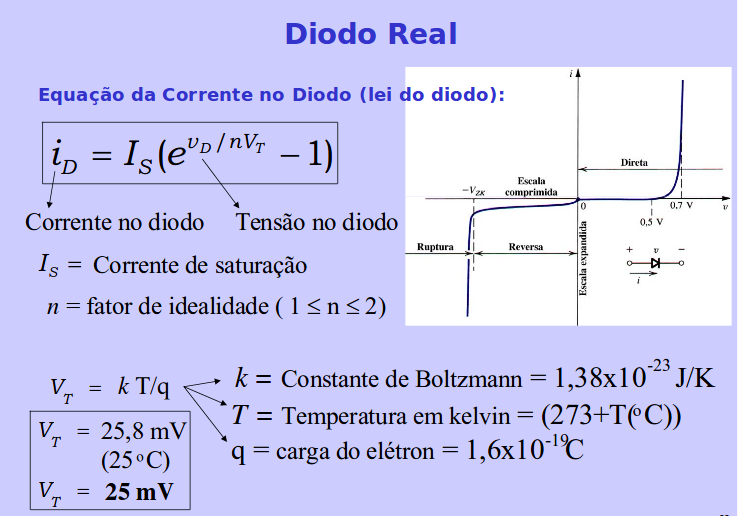
\includegraphics[scale=0.5]{images/img1.png}
    Imagem 1: Modelo do diodo real
\end{center}

\section{Estrutura do projeto}
O trabalho começa no FPGA, onde iremos implementar um algorítmo de Aproximações Sucessivas, i.e um conversor analógico digital. A saída do FPGA (pinos 3.3V) mandando sinais para uma rede R2R

\section{Simulação Conversor AD}
Usaremos as redes R-2R, que nos fornecem a possibilidade de conseguir variar níveis de tensão de acordo com as disposições dos resistores, i.e usando uma rede R-2R de 7 bits obteremos: 2(elevado)7 128 valores possiveis pra dividir a tensão de entrada. Como queremos medir de 0 100 graus com passo de 1 grau, então um R-2R de 7 bits será suficiente. Na saída da rede R2R iremos ter um ampop comparador para pegar esses valores de tensão e iremos "filtra-lo". Assim, teremos uma relação tensão-temperatura.


\end{document}
